\documentclass[12pt,a4paper,oneside,onecolumn]{article}

\usepackage[spanish,es-noshorthands]{babel}
\usepackage{epsfig}
\usepackage[latin1]{inputenc}
\usepackage{amsmath}
\usepackage{amsfonts}
\usepackage{amssymb}
%\usepackage{mathabx}  Compila pero borra el pdf?
\usepackage{array}
\usepackage[left=1.8cm, right=1.8cm, top=2.50cm, bottom=2.5cm]{geometry}
\usepackage{hyperref}
\usepackage{color}
\usepackage{fancyhdr}
\usepackage{listings}
\usepackage{xcolor}
\usepackage[smartEllipses]{markdown}

\pagestyle{fancy}

\fancyhead{}
\fancyfoot{}

\setlength{\headsep}{0.4cm}
\setlength{\footskip}{1.6pt}
\setlength{\parindent}{0pt}
\setlength{\extrarowheight}{1.5pt}


\lhead{Proyectos II}
\rhead{Javier Orti}
\renewcommand*\headrulewidth{0.4 pt}
\lfoot{\vspace{0.45cm}File Upload}
\cfoot{\vspace{0.01cm}\rule{\linewidth}{0.4pt}}
\rfoot{\vspace{0.45cm} P\'ag. \thepage}

\renewcommand{\labelitemi}{$\bullet$}
\renewcommand{\labelenumi}{\theenumi)}
\renewcommand\spanishtablename{Tabla}

\decimalpoint

\headheight 16.7pt 
\textheight 715pt 

\parskip 8pt  

\hypersetup{
	colorlinks=true,
	linkcolor=blue,
	filecolor=magenta,      
	urlcolor=cyan,
}

% Python code settings
\definecolor{codegreen}{rgb}{0,0.6,0}
\definecolor{codegray}{rgb}{0.5,0.5,0.5}
\definecolor{codepurple}{rgb}{0.58,0,0.82}
\definecolor{backcolour}{rgb}{0.95,0.95,0.92}

\lstdefinestyle{mystyle}{
	backgroundcolor=\color{backcolour},   
	commentstyle=\color{codegreen},
	keywordstyle=\color{magenta},
	numberstyle=\tiny\color{codegray},
	stringstyle=\color{codepurple},
	basicstyle=\ttfamily\footnotesize,
	breakatwhitespace=false,         
	breaklines=true,                 
	captionpos=b,                    
	keepspaces=true,                 
	numbers=left,                    
	numbersep=5pt,                  
	showspaces=false,                
	showstringspaces=false,
	showtabs=false,                  
	tabsize=2
}

\lstset{style=mystyle}

\usepackage[shortlabels]{enumitem}
\usepackage{cancel}

\begin{document} 
    \section{}
    Una vulnerabilidad de file upload es aquella en la que un servidor permite al cliente enviar archivos sin la validaci\'on suficiente, y por tanto, el cliente de forma maliciosa puede aprovecharse para enviar un archivo malicioso con side scripts que puedan incluso darle acceso remoto al servidor.
    \section{}
    Los pasos a seguir variar\'an mucho seg\'un las medidas que tome el servidor, pero se resumen en subir el archivo pasando los filtros inciales(por ejemplo la extensi\'on del archivo si est\'a limitada) y conseguir que se ejecute en remoto.
    \section{}
    Algunos de los m\'as importantes son:
    \begin{enumerate}[a)]
        \item
        \underline {Segregar los uploads:} en la mayor\'ia de aplicaciones querremos archivos como im\'agenes, v\'ideos, documentos de texto... Y estos normalmente se pueden guardar en bases de datos en el cloud, por lo que no tienen contacto directo con el backend.
        \item
        \underline{Asegurarnos de que no sean ejecutables:} por ejemplo en los sistemas Unix, con el comando \emph{chmod} podr\'iamos asegurar que el flag x(executable) est\'e desactivado.
        \item
        \underline{Renombrar los archivos.}
        \item
        \underline{Validar el Content-Type Header.}
        \item
        \underline{Validar el tama\~no del archivo.} Esto nos sirve incluso para algunos ataques muy b\'asicos de DDoS que consisten en subir archivos enormes.
        \underline{Blacklist:} Consiste en prohibir que ciertos tipos de strings sean enviados al servidor.
        \item
        \underline{Whitelist:} Lo contrario al anterior, consiste en \'unicamente permitir que ciertos tipos de strings sean enviados al servidor.
    \end{enumerate}
    
    \section{}
    Un ejemplo b\'asico pero efectivo ser\'ia por ejemplo si nos requieren una imagen tipo \emph{jpg}, nosotros enviamos un archivo de tipo \emph{shell.php.jpg} que se ejecutar\'a m\'as tarde como un script de php.
    Para pasar algunas blacklist, podemos utilizar extensiones de archivo diferentes como \emph{.pht, .phtml, .php3, .php4, .php5, .php6, .inc} para php o \emph{.jspx, .jspf, .jsw, .jsv} para web shell.
    En el caso de las whitelist, el ejemplo anterior de la doble extensi\'on para servidores que lo acepten como Apache, o probar un null byte injection, que a veces ser\'a ignorado como shell.php\%00.jpg o shell.php\textbackslash x00.jpg.
    
    \section{}
    Una webshell son scripts que se lanzan en servidores web y que se explotan en hacking como vectores de ataque. Un ejemplo son servidores que utilicen el lenguaje php. Algunos ejemplos son el China Chopper, C99 o B374K.
	
	\section{}
	Ahora vamos con los files uploads. En dificultad media:
	Creamos una 'imagen' con extension .html.jpg tal que as\'i, y la subimos al servidor:
	\begin{lstlisting}[language = html]
    <html>
    <body>
    	
    	<script>
    		alert("te han hackeado");
    	</script>
    
    </body>
    </html>
    \end{lstlisting} 
    \begin{figure}[!h]
		\centering
		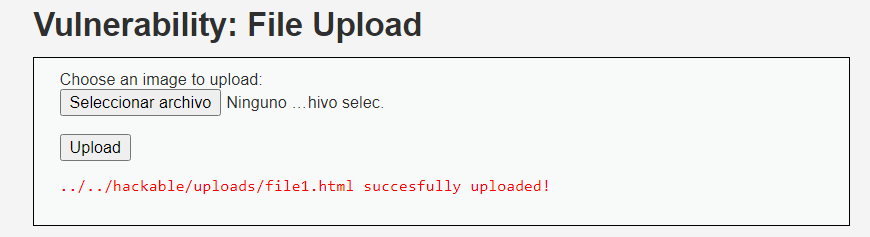
\includegraphics[scale=0.6]{fileUp2.png}
		\caption{}
		\label{fig:2}
	\end{figure}
	Una vez subida, si vamos a la ruta que nos devuelve la p\'agina, podremos ejecutar el script. Hay que tener en cuenta que en la realidad obviamente la web no nos va a decir la ruta.
    
\end{document}